% !TEX root = ../main.tex
\section{Ejercicio propuesto 2: comparación experimental}

\subsection{Diseño y metodología de medición}
Se estudiaron siete tamaños ($16$--$1024$ bits) y se generaron $30$ probables primos por tamaño. Para la comparación se prepararon $8$ candidatos aceptados y $8$ compuestos impares por tamaño. Solo los aceptados de $16$ y $32$ bits se verificaron también por división de prueba. Las semillas de generación, comparación y simulación fueron \texttt{20260701}, \texttt{20260702} y \texttt{20260703}.

Las mismas entradas y $20$ bases preseleccionadas alimentaron Fermat y Miller--Rabin con $1$, $5$, $10$ y $20$ rondas; la división se midió solo hasta $32$ bits. Se hicieron siete repeticiones por caso con \texttt{perf\_counter\_ns()}, sin selección de bases, impresión ni escritura durante el cronometraje. Se registraron tiempos y operaciones. El precribado se desactivó \emph{solo} para comparar pruebas; en generación permaneció activo.

\subsection{Comparación de tiempo y operaciones}
Las medianas sobre candidatos aceptados (Tabla \ref{tab:tiempos}) y la dispersión de siete mediciones de un caso (Tabla \ref{tab:dispersion}) no son la misma estadística. Los registros y bases constan en \path{python/results/comparacion_metodos.csv} y \path{python/results/entradas_y_bases.csv}.
\begin{table}[H]\centering\small
\caption{Tiempo mediano por prueba sobre probables primos (µs)}
\label{tab:tiempos}
\begin{tabular}{rrrrrr}\toprule
Bits & División & Fermat 20 & MR 1 & MR 5 & MR 20 \\
\midrule
16 & 17.1 & 173.4 & 14.2 & 56.7 & 209.3 \\ 
32 & 6177.6 & 564.2 & 33.1 & 149.2 & 606.2 \\ 
64 & -- & 1366.2 & 70.8 & 372.6 & 1319.2 \\ 
128 & -- & 3560.7 & 149.7 & 927.5 & 2947.2 \\ 
256 & -- & 10164.4 & 434.1 & 2639.2 & 10243.0 \\ 
512 & -- & 44926.6 & 2300.7 & 10997.1 & 44781.4 \\ 
1024 & -- & 221081.4 & 10763.3 & 53382.4 & 228012.8 \\ 
\bottomrule\end{tabular}\end{table}

\begin{table}[H]\centering\small
\caption{Mínimo, mediana y máximo de siete pruebas sobre una misma entrada ($\mu$s)}
\label{tab:dispersion}
\begin{tabular}{rlrrr}\toprule
Bits & Método & Mínimo & Mediana & Máximo \\
\midrule
16 & División & 17.6 & 17.9 & 19.0 \\
16 & MR 20 & 207.3 & 217.4 & 241.8 \\
32 & División & 3746.7 & 4249.9 & 13950.4 \\
32 & MR 20 & 406.6 & 650.2 & 672.7 \\
1024 & MR 20 & 209706.7 & 224301.2 & 226631.5 \\
\bottomrule\end{tabular}\end{table}

\noindent\textbf{Lectura cuantitativa del costo y error.} Para 1024 bits, la mediana de Miller--Rabin con 20 rondas fue 228012.8~$\mu$s frente a 10763.3~$\mu$s con una ronda (razón 21.2); Fermat con 20 rondas tomó 221081.4~$\mu$s. El compuesto 341 presentó 48 mentirosos fuertes entre 338 bases válidas: $p_{341}=0.1420$. El tiempo medido de Fermat no resuelve sus falsos positivos para Carmichael; cero errores observados tras varias rondas no implica probabilidad cero.\par


\begin{figure}[H]\centering
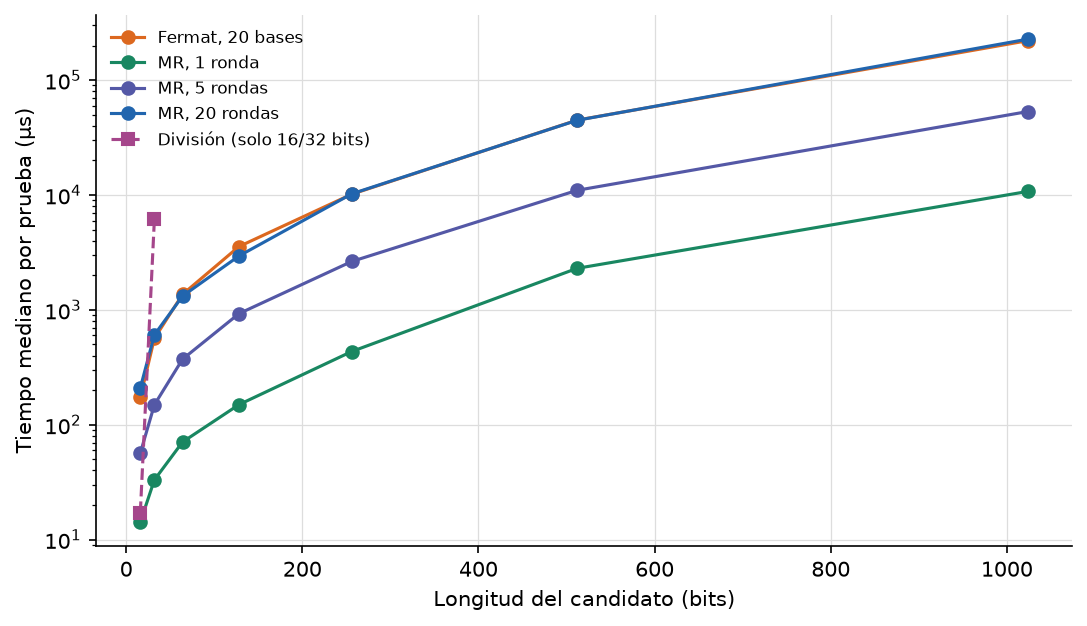
\includegraphics[width=.88\textwidth]{fig1_tiempo_vs_bits.png}
\caption{Tiempo mediano por prueba y longitud binaria; escala temporal logarítmica. La división se ejecuta solo hasta $32$ bits.}\label{fig:tiempo}
\end{figure}
\begin{figure}[H]\centering
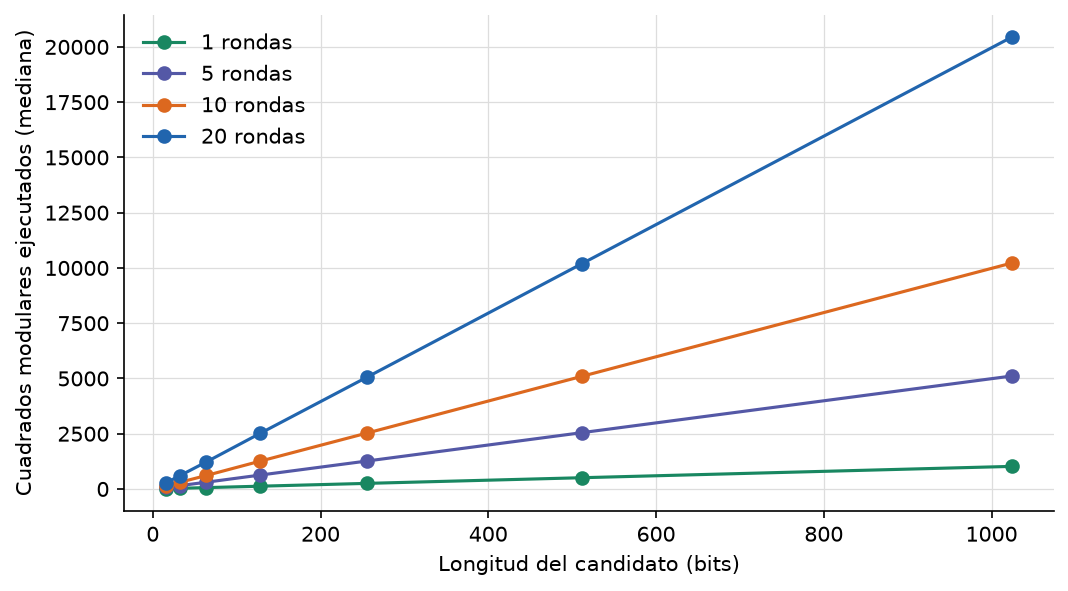
\includegraphics[width=.88\textwidth]{fig2_cuadrados_vs_bits.png}
\caption{Cuadrados modulares efectivamente realizados por Miller--Rabin con $1$, $5$, $10$ y $20$ rondas.}\label{fig:cuadrados}
\end{figure}
Un testigo detiene las rondas de un compuesto; en un candidato aceptado se completan. El costo por prueba no equivale al costo de buscar un probable primo.

\subsection{Generación y precribado}
La Tabla \ref{tab:generacion} presenta candidatos, descartes y tiempo; los $210$ registros individuales están en \path{python/results/generacion_210_probables_primos.csv}.
\begin{table}[H]\centering\small
\caption{Generación de 30 probables primos por longitud binaria}
\label{tab:generacion}
\begin{tabular}{rrrrrr}\toprule
Bits & Candidatos & Media & Mediana & Descartes & Tiempo med. (ms) \\
\midrule
16 & 169 & 5.63 & 5.0 & 139 & 0.220 \\
32 & 371 & 12.37 & 10.5 & 310 & 0.720 \\
64 & 652 & 21.73 & 16.5 & 537 & 1.367 \\
128 & 970 & 32.33 & 22.5 & 806 & 3.181 \\
256 & 1840 & 61.33 & 40.5 & 1541 & 10.599 \\
512 & 5307 & 176.90 & 97.5 & 4445 & 69.182 \\
1024 & 12870 & 429.00 & 314.5 & 10833 & 802.315 \\
\bottomrule\end{tabular}\end{table}

\noindent\textbf{Lectura cuantitativa de la generación.} Para 1024 bits se necesitaron 12870 candidatos para 30 probables primos (media 429.00, mediana 314.5); el precribado descartó 10833 (84.2\%). La referencia asintótica es 354.9 candidatos impares por primo. Para 512 bits, la media observada fue 176.90 frente a 177.4 estimados. Las diferencias con la aproximación pueden reflejar variación muestral; por sí solas no prueban ni descartan errores de primalidad.\par

\begin{figure}[H]\centering
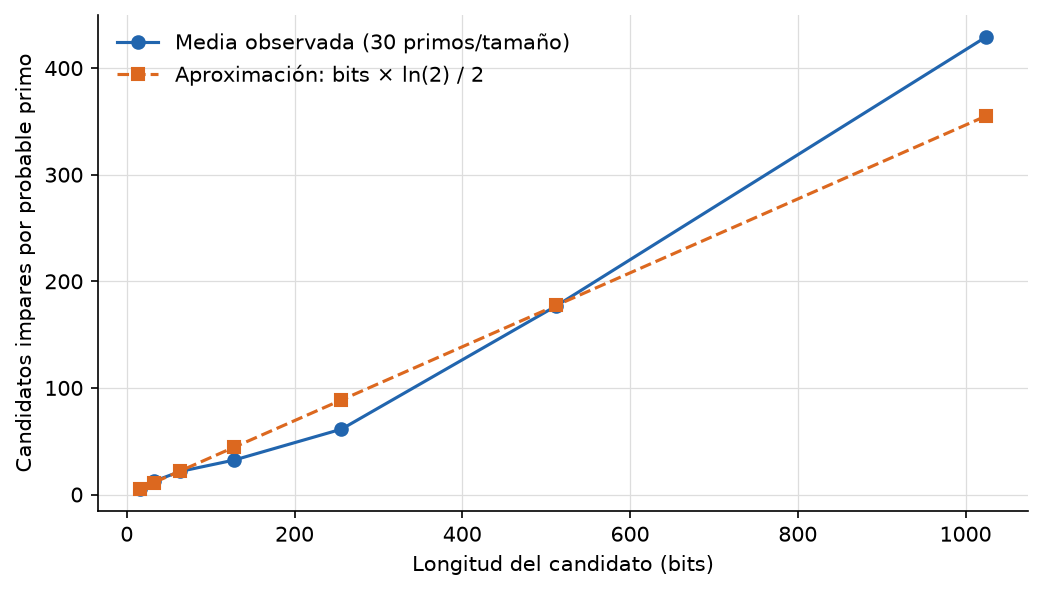
\includegraphics[width=.88\textwidth]{fig3_candidatos_vs_bits.png}
\caption{Candidatos impares por probable primo: media de $30$ muestras y aproximación $L\ln(2)/2$.}\label{fig:candidatos}
\end{figure}
El precribado reduce trabajo, no altera la densidad prima de los candidatos originales.

\subsection{Testigos, mentirosos fuertes y probabilidad de error}
La Tabla \ref{tab:mentirosos} cuenta testigos y mentirosos fuertes; \path{python/results/clasificacion_bases.csv} identifica cada base pequeña. Para un compuesto fijo con fracción $p_n$ de mentirosos, $p_n^r$ es la probabilidad de aceptar $r$ bases uniformes independientes; $4^{-r}$ es solo su cota superior.

La simulación usa bases clasificadas de $25$, $91$, $121$, $341$ y $561$; no mide tiempo. Cero falsos positivos en una muestra finita no demuestra error imposible. Fermat carece de una cota análoga ante números de Carmichael.
\begin{table}[H]\centering\small
\caption{Testigos y mentirosos fuertes: bases válidas de compuestos seleccionados}
\label{tab:mentirosos}
\begin{tabular}{rrrrr}\toprule
$n$ & Bases & Testigos & Mentirosos & Fracción \\
\midrule
25 & 22 & 20 & 2 & 0.0909 \\
91 & 88 & 72 & 16 & 0.1818 \\
121 & 118 & 110 & 8 & 0.0678 \\
221 & 218 & 214 & 4 & 0.0183 \\
341 & 338 & 290 & 48 & 0.1420 \\
561 & 558 & 550 & 8 & 0.0143 \\
\bottomrule\end{tabular}\end{table}

\begin{table}[H]\centering\small
\caption{Aceptación empírica y exacta de compuestos para 3000 ensayos por fila}
\label{tab:error}
\begin{tabular}{rrrrrr}\toprule
$n$ & Rondas & Aceptados & Frecuencia & Exacta $p_n^r$ & Cota $4^{-r}$ \\
\midrule
25 & 1 & 281 & 0.0937 & 0.0909 & 0.25 \\
25 & 5 & 0 & 0 & 6.21e-06 & 0.000977 \\
25 & 20 & 0 & 0 & 1.49e-21 & 9.09e-13 \\
341 & 1 & 413 & 0.138 & 0.142 & 0.25 \\
341 & 5 & 0 & 0 & 5.78e-05 & 0.000977 \\
341 & 20 & 0 & 0 & 1.11e-17 & 9.09e-13 \\
561 & 1 & 38 & 0.0127 & 0.0143 & 0.25 \\
561 & 5 & 0 & 0 & 6.06e-10 & 0.000977 \\
561 & 20 & 0 & 0 & 1.35e-37 & 9.09e-13 \\
\bottomrule\end{tabular}\end{table}

\begin{figure}[H]\centering
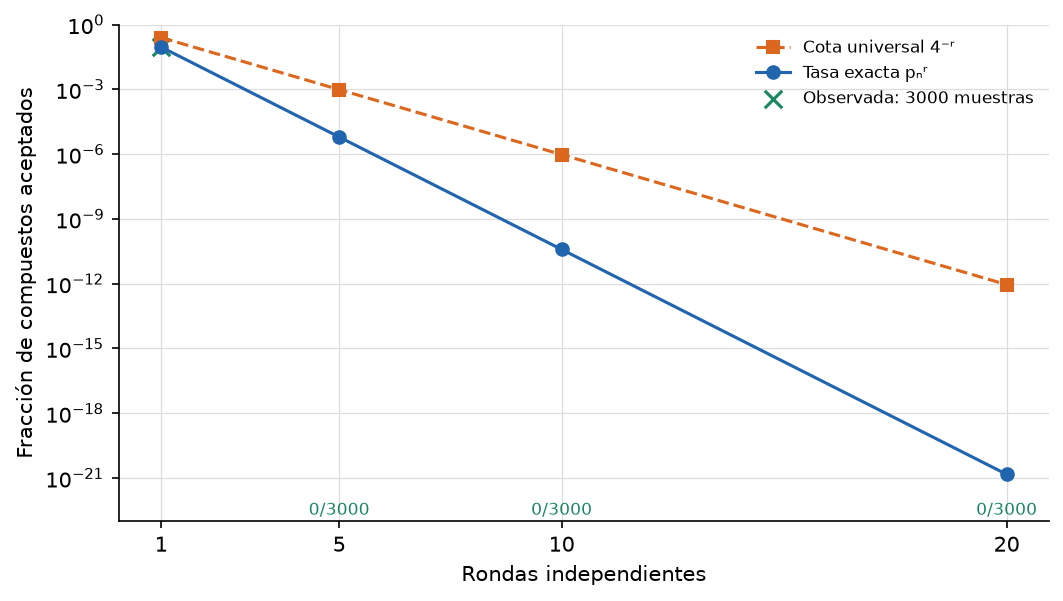
\includegraphics[width=.88\textwidth]{fig4_error_empirico.png}
\caption{Compuesto $25$: tasa exacta $p_n^r$, cota $4^{-r}$ y $3000$ ensayos por número de rondas. Los ceros observados se anotan como $0/3000$, no como probabilidades positivas.}\label{fig:error}
\end{figure}
